\documentclass[tikz, border=10pt]{standalone}
\begin{document}
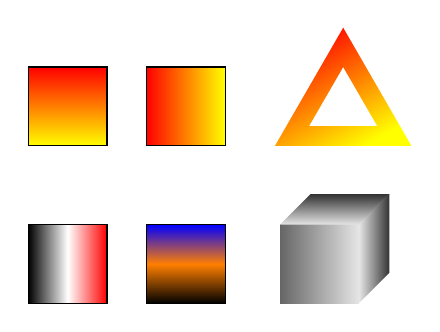
\begin{tikzpicture}
    \begin{scope}
        \shadedraw[top color=red, bottom color=yellow] (0, 0) rectangle (1, 1);
        \shadedraw[left color=red, right color=yellow]  (1.5, 0) rectangle (2.5, 1);
    \end{scope}
    \begin{scope}[xshift=4cm, yshift=0.5cm]
        \shade[top color=red, bottom color=yellow, shading angle=30]
        (90:1) -- (210:1) -- (330:1) -- cycle
        (90:0.5) -- (330:0.5) -- (210:0.5) -- cycle;
    \end{scope}

    \begin{scope}[yshift=-2cm, xshift=3.2cm]
        \shade[left color=black!60, right color=black!10]
        (0,0,0) -- (1,0,0) -- (1,1,0) -- (0,1,0);
        \shade[left color=black!10, right color=black!80]
        (1,0,0) -- (1,0,-1) -- (1,1,-1) -- (1,1,0);
        \shade[bottom color=black!10, top color=black!80]
        (0,1,0) -- (0,1,-1) -- (1,1,-1) -- (1,1,0);
    \end{scope}

    \begin{scope}[yshift=-2cm]
        \shadedraw[left color=black, right color=red, middle color=white] (0, 0) rectangle (1, 1);
        \shadedraw[bottom color=black, top color=blue, middle color=orange]  (1.5, 0) rectangle (2.5, 1);
    \end{scope}
\end{tikzpicture}
\end{document}